% Author: Hadrian Lau
% Website: https://www.hadrian.cc
% License: LaTeX Project Public License (LPPL)

\documentclass[a4paper,12pt]{article}

% Packages
\usepackage[utf8]{inputenc}
\usepackage[english]{babel}
\usepackage{amsmath, amsthm, amssymb, amsfonts}
\usepackage{graphicx}
\usepackage{setspace}
\usepackage{geometry}
\usepackage{float}
\usepackage{framed}
\usepackage[dvipsnames,svgnames]{xcolor}
\usepackage[most]{tcolorbox}
\usepackage{thmtools}
\usepackage{indentfirst}
\usepackage{parskip}
\usepackage{chemfig}
\usepackage{pgfplots}
\usepackage[version=4,arrows=pgf-filled,mathfontname=mathsf]{mhchem}
\usepackage{fancyhdr}
\usepackage{titlesec}
\usepackage{xpatch}
\usepackage{blindtext}
\usepackage{hyperref}
\usepackage{empheq}
\usepackage{apacite}

% Settings
\pgfplotsset{width=15cm,compat=1.18}
\geometry{margin=1in}
\setstretch{1.5}
\newcommand{\HRule}[1]{\rule{\linewidth}{#1}}

% Box equations
\makeatletter
\newcommand{\colorboxed}[1]{\fcolorbox{DarkSeaGreen}{DarkSeaGreen!20}{\m@th$\displaystyle#1$}}
\xpatchcmd{\@Aboxed}{\boxed}{\colorboxed}{}{}
\makeatother

% Note sections
\makeatletter
\NewDocumentCommand{\mynote}{+O{}+m}{%
	\begingroup
	\tcbset{%
		noteshift/.store in=\mynote@shift,
		noteshift=1.5cm
	}
	\begin{tcolorbox}[nobeforeafter,
		enhanced,
		sharp corners,
		toprule=1pt,
		bottomrule=1pt,
		leftrule=0pt,
		rightrule=0pt,
		colback=DarkSeaGreen!20,
		#1,
		left skip=\mynote@shift,
		right skip=\mynote@shift,
		overlay={\node[right] (mynotenode) at ([xshift=-\mynote@shift]frame.west) {\textbf{Note:}} ;},
		]
		#2
	\end{tcolorbox}
	\endgroup
}
\makeatother

% Header and Footer
\pagestyle{fancy}
\fancyhf{}
\fancyhead[L]{Pendulum and Projectile Motion} % HERE
\fancyhead[R]{\thepage}

% Document
\begin{document}
	
	% Front page
	\title{ \normalsize \textsc{}
		\\ [2.0cm]
		\HRule{1.5pt} \\
		\LARGE \textbf{
			\uppercase{Pendulum and Projectile Motion} % HERE
			\HRule{2.0pt} \\ [0.6cm] 
			\LARGE{SPH3U Unit 1 Lab} % HERE
			\vfill
		}
	}
	\date{}
	\author{
		\textbf{Hadrian Lau Yiu Hei} \\ 
		\textbf{Ms. Rashmi Shroff}\\
		Sin Chi Lam, Jae-Hee Han, Sadan Ahmed Shaikh, Brinstan Lo, Junho Song \\
		26th September, 2025\\ %HERE
		\href{https://github.com/udontur/latex/blob/main/sph3u-u01}{{\color{blue}\underline{\LaTeX\, document code}}}
	}
	\maketitle
	\thispagestyle{empty}
	
	\newpage

	% Table of content
	\setcounter{page}{1}
	\tableofcontents
	\newpage
	
	% Content
	\section{Pendulum Motion}
	A steel ball, attached to a 33cm long string, is dropped from a $5^{\circ}$ angle and swings freely. We tracked the time it takes for 10 oscillations to occur using a $8\times$ slow-motion camera \cite{cite3}. 
	
	\subsection{Raw data}
	Length of pendulum wire: $L=33\text{cm}=0.33\text{m}$\\
	Initial angular displacement: $\theta=5^\circ$ to the right\\
	
	\subsubsection{Trials}
	We did a total of 3 trials, each measuring the time for 10 pendulum oscillations to occur:
	\begin{align*}
		t_1&=11.66\text{s}\\
		t_2&=11.85\text{s}\\
		t_3&=11.65\text{s}
	\end{align*}\\
	\subsection{Trial calculations}
	The average time for 10 oscillations are:
	\begin{align*}
		t_{10avg}&=\frac{11.66\text{s}+11.85\text{s}+11.65\text{s}}{3}\\
		&=\frac{35.16\text{s}}{3} \\
		t_{10avg}&=11.72\text{s}\\
	\end{align*}
	
	Hence, the average time for 1 oscillation to occur is:
	\begin{align*}
		t_{avg}&=\frac{11.72\text{s}}{10}\\
		\Aboxed{t_{avg}&=1.17\text{s}}
	\end{align*}
	
	\subsection{Theoretical time}
	We can calculate the theoretical time for each oscillation to occur using the simple harmonic motion equation:
	\begin{align*}
		t_{the}&=2\pi\times\sqrt{\frac{L}{g}}\\
		&=2\pi\times\sqrt{\frac{0.33\text{m}}{9.81\text{m}/\text{s}^2}}  \\
		&=2\pi\times\sqrt{0.034\text{s}^2}\\
		&=2\pi\times 0.183\text{s} \\
		\Aboxed{t_{the}&=1.15\text{s}}
	\end{align*} 
	\newpage
	\subsection{Error sources}
	There is a very small difference between our actual time and theoretical time: 
	\begin{align*}
		\Delta&=1.17\text{s}-1.15\text{s} \\
		&=0.02\text{s}\\
	\end{align*}
	This marginal time difference of 20 milliseconds can be caused by errors like:
	\begin{itemize}
		\item Human error: The measurement of string length (The bar and the steel ball is in the way when we try to measure the string length), oscillation time, and calculations are all rounded. Precision is loss during this process. 
		\item Air resistance: The steel ball and string experiences air resistance, which slows down the pendulum as heat energy from the friction between air and the two objects are transferred to the surrounding.
	\end{itemize}
	\subsection{Experiment optimization}
	We can optimize the experiment by:
	\begin{itemize}
		\item Fixed string length: Attaching a pre-cut string ensures the length to be more accurate and stable throughout the experiment, preventing gear slipping and interference during measurement. 
		\item High-accuracy slow-motion camera: A slow-motion camera with high accuracy, such as a 32× slow-motion camera, enhances time measurement by increasing the time resolution.
	\end{itemize}
	\newpage
	
	\section{Projectile motion}
	A steel ball is projected forward from a ramp. The ball's trajectory is tracked by a grid plane and captured using a 8$\times$ slow-motion camera.
	
	\subsection{Raw data}
	Each grid's length: 2cm=0.2m\\
	Each grid's width: 2cm=0.2m
	
	We can compile the following data using the 8$\times$ slow-motion video:
	\bigskip
	\bigskip
	\begin{center}
		\begin{tabular}{ |c|c|c| } 
			\hline
			t (s) & $\vec{\Delta d_x}$ (m [$\rightarrow$]) & $\vec{\Delta d_y}$ (m [$\uparrow$]) \\ 
			\hline\hline
			0.00s & 0.00m & 0.20m\\
			\hline 
			0.03s & 0.02m & 0.19m \\ 
			\hline
			0.06s & 0.04m & 0.17m \\
			\hline
			0.09s & 0.06m & 0.14m \\
			\hline
			0.12s & 0.08m & 0.10m \\
			\hline
			0.15s & 0.10m & 0.05m \\
			\hline
			0.18s & 0.12m & 0.00m \\
			\hline
		\end{tabular} 
	\end{center}
	\bigskip
	\bigskip
	\bigskip
	\mynote{We measured everything using the steel ball's bottom.}
	\mynote{The slow-motion video is recording at 8 times slower than real time (240 fps to 30 fps). }
	
	\newpage
	
	\subsection{Calculations}
	All calculations are based on the table of values. 
	\subsubsection{Total Displacement (x-axis)}
	The total displacement in the x-axis:
	\begin{align*}
		\vec{\Delta d}_x&=\vec{\Delta d}_{xf}-\vec{\Delta d}_{xi}\\
		&=0.12 \text{m}\;[\rightarrow]-0.0 \text{m}\; [\rightarrow]\\
		\Aboxed{\vec{\Delta d}_x&=0.12\text{m}\; [\rightarrow]}
	\end{align*}
	\subsubsection{Total Displacement (y-axis)}
	The total displacement in the y-axis
	\begin{align*}
		\vec{\Delta d}_y&=\vec{\Delta d}_{yf}-\vec{\Delta d}_{yi}\\
		&=0.00 \text{m}\; [\uparrow]-0.20 \text{m}\; [\uparrow]\\
		&=-0.20\text{m}\; [\uparrow]\\
		\Aboxed{\vec{\Delta d}_y&=0.20\text{m}\; [\downarrow]}
	\end{align*}
	\subsubsection{Initial Velocity \& Final Velocity (x-axis)}
	According to the laws of projectile motion, $\vec{v_{ix}}=\vec{v_{fx}}$.
	\begin{align*}
		\vec{\Delta d}_x&=\vec{v_x}\times \Delta t\\
		0.12\text{m}\; [\rightarrow]&=\vec{v_x} \times 0.18\text{s}\\
		\vec{v_x}&=\frac{0.12\text{m}\; [\rightarrow]}{0.18\text{s}}\\
		      &=0.67\text{m}/\text{s}\;[\rightarrow]\\
		\Aboxed{\vec{v_{ix}}=\vec{v_{fx}}&=0.67\text{m}/\text{s}\;[\rightarrow]}
	\end{align*}
	\subsubsection{Initial Velocity (y-axis)}
	Since we did not push the steel ball downwards, gravity is the only force that affects it. Hence, there is no initial velocity:
	\begin{align*}
		\Aboxed{\vec{v_{iy}}&=0\text{m}/\text{s}\;[\emptyset]}\\
	\end{align*}
	\subsubsection{Final Velocity (y-axis)}
	The final velocity in the y-axis:
	\begin{align*}
		\vec{\Delta d}_y&=\Delta t\left(\vec{v}_{fy}-\frac{1}{2}\vec{a}_y\Delta t\right)\\
		0.20\text{m}\;[\downarrow]&=0.18\text{s}\left(\vec{v}_{fy}-\frac{1}{2}\left(9.81\text{m}/\text{s}^2\;[\downarrow]\right)0.18\text{s}\right)\\
		\frac{0.20\text{m}\;[\downarrow]}{0.18\text{s}}&=\vec{v}_{fy}-\frac{1}{2}\times9.81\text{m}/\text{s}^2\;[\downarrow]\times0.18\text{s}\\
		1.1\text{m}/\text{s}\;[\downarrow]&=\vec{v}_{fy}-0.88\text{m}/\text{s}\;[\downarrow]\\
		\Aboxed{\vec{v}_{fy}&=1.98\text{m}/\text{s}\;[\downarrow]}
	\end{align*}
	\newpage
	\subsection{Position-Time graph}
	We can plot a graph using the table of values, where the displacement is on the y-axis ($\vec{\Delta d}_y$) in $\text{m} \,[\rightarrow]$ (meters), and the time (t) in s (seconds) is on the x-axis:
	\bigskip
	\bigskip
	\begin{center}
		\begin{tabular}{ |c|c| } 
			\hline
			t (s) & $\vec{\Delta d_y}$ (m [$\uparrow$]) \\ 
			\hline\hline
			0.00s & 0.20m \\
			\hline 
			0.03s & 0.19m \\ 
			\hline
			0.06s & 0.17m \\
			\hline
			0.09s & 0.14m \\
			\hline
			0.12s & 0.10m \\
			\hline
			0.15s & 0.05m \\
			\hline
			0.18s & 0.00m \\
			\hline
		\end{tabular} 
	\end{center}
	\bigskip
	\bigskip
	\bigskip
	\subsubsection{Theoretical displacement equation}
	We included the theoretical graph as a comparison for error sources:
	\begin{align*}
		\vec{\Delta d}_y&=\Delta t\left(\vec{v}_{iy}+\frac{1}{2}\vec{a}_y\Delta t\right)\\
		&=\Delta t\left(0+\frac{1}{2}(-9.81 \text{m}/\text{s}^2\;[\uparrow])\Delta t\right)\\
		\vec{\Delta d}_y&=-4.905 \text{m}/\text{s}^2\;[\uparrow]\times\Delta t^2\\
	\end{align*}
	Since we are dropping from a height of 0.20m, we get the following equation:
	\begin{align*}
		\vec{\Delta d}_y&=0.20-4.905 \text{m}/\text{s}^2\;[\uparrow]\times\Delta t^2\\
		\Aboxed{\vec{\Delta d}_y&=0.2-4.905t^2}
	\end{align*}
	
	\subsubsection{Position-Time graph}
	\begin{center}
		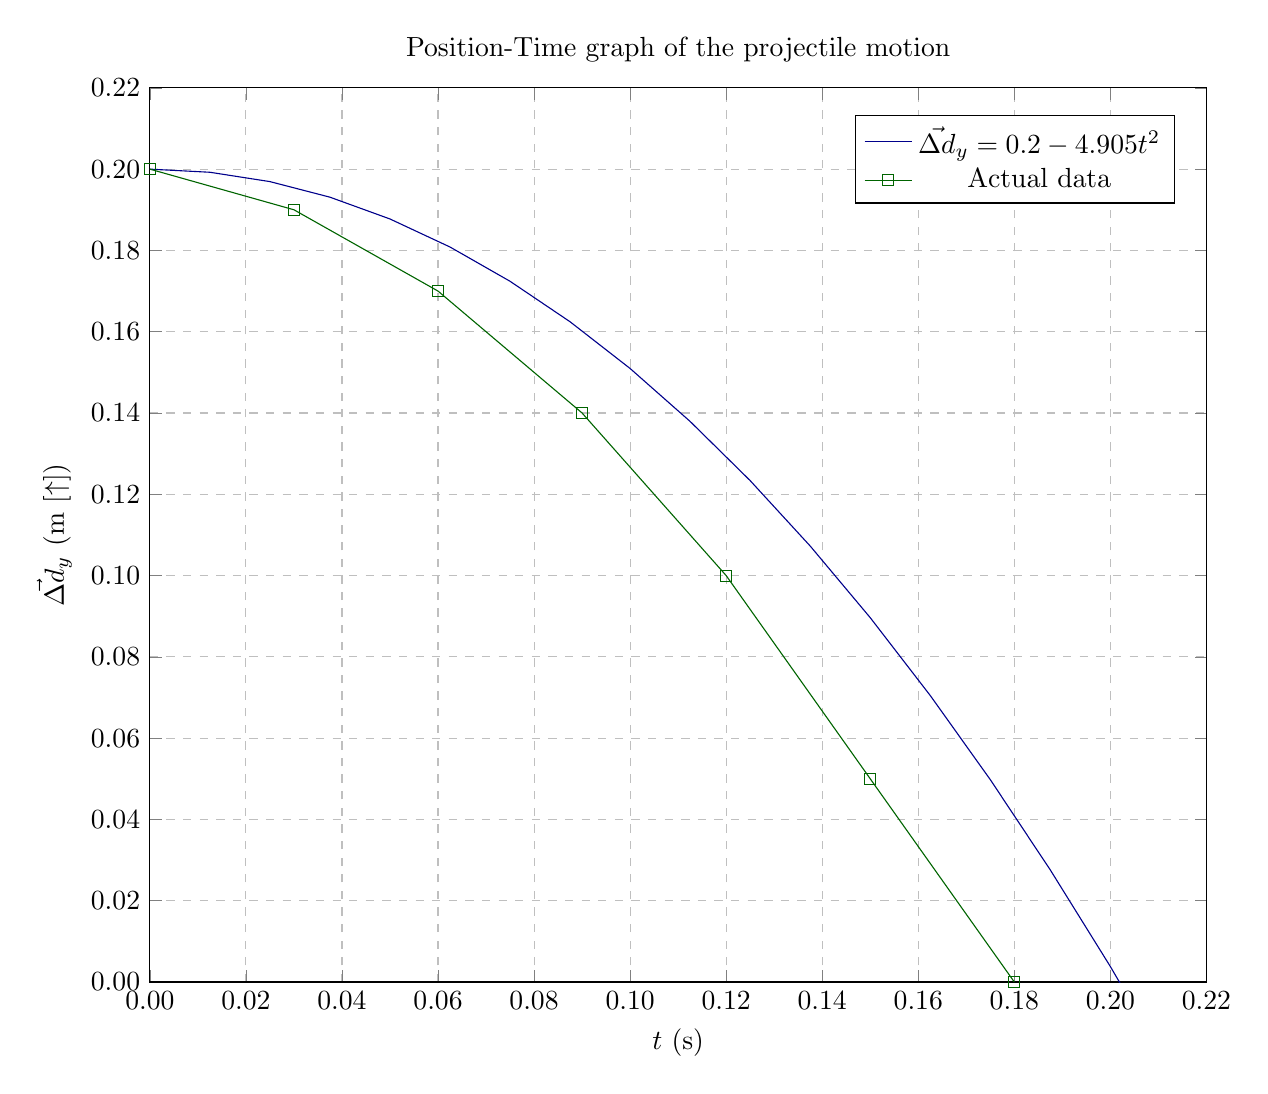
\begin{tikzpicture}
			\begin{axis} [
				title={Position-Time graph of the projectile motion},
				xlabel={$t$ (\text{s})},
				ylabel={$\vec{\Delta d}_y$ (\text{m} [$\uparrow$])},
				xmin=0, xmax=0.22,
				ymin=0, ymax=0.22,
				y tick label style={/pgf/number format/fixed,
					/pgf/number format/fixed zerofill={true}},
				x tick label style={/pgf/number format/fixed,
					/pgf/number format/fixed zerofill={true}},
				xtick distance=0.02,
				ytick distance=0.02,
				ymajorgrids=true,
				xmajorgrids=true,
				legend pos=north east,
				grid style=dashed,
				]	
				\addplot[
				color=DarkBlue,
				domain=0:0.3,
				] {
					0.2-4.905*x*x
				};
				\legend{$\vec{\Delta d}_y=0.2-4.905t^2$, Actual data}
				\addplot[
				color=DarkGreen,
				mark=square,
				] coordinates {
					(0,0.2)(0.03,0.19)(0.06,0.17)(0.09,0.14)(0.12,0.10)(0.15,0.05)(0.18,0)
				};
			\end{axis}
		\end{tikzpicture}
	\end{center}
	\newpage
	\subsection{Velocity-Time graph}
	There are no raw data for the velocity of the steel ball. Hence, we need to calculate the equation for the velocity by taking the derivative of the position-time curve of best fit equation.
	\subsubsection{Velocity-Time equation}
	By entering the position-time data in Google Sheets, we get the following equation for the curve of best fit of the position-time graph \cite{cite2}:
	\begin{align*}
	V(t)=-4.89t^2-0.25t+0.201 
	\end{align*}
	
	Take the derivative of $V(t)$ \cite{cite1}:
	\begin{align*}
		V'(t)&=\frac{d}{dt}\left[-4.89t^2-0.25t+0.201\right]\\
		&=\frac{d}{dt}[-4.89t^2]-\frac{d}{dt}[0.25t]+\frac{d}{dt}[0.201]\\
		&=-4.89(2t)-0.25+0\\
		\Aboxed{V'(t)&=-9.78t-0.25}
	\end{align*}
	\subsubsection{Theoretical velocity-time equation}
	We included the theoretical graph as a comparison for error sources:
	\begin{align*}
		\vec{a}_y&=\frac{\vec{v}_{fy}-\vec{v}_{iy}}{\Delta t}\\
		-9.81\text{m}/\text{s}^2\;[\uparrow]&=\frac{\vec{v}_{fy}-0}{\Delta t}\\
		-9.81\text{m}/\text{s}^2\;[\uparrow]\times\Delta t&=\vec{v}_{fy}\\
		\Aboxed{\vec{v}_y&=-9.81t}lam_2025_what
	\end{align*}
	
	\subsubsection{Velocity-Time graph}
	\begin{center}
		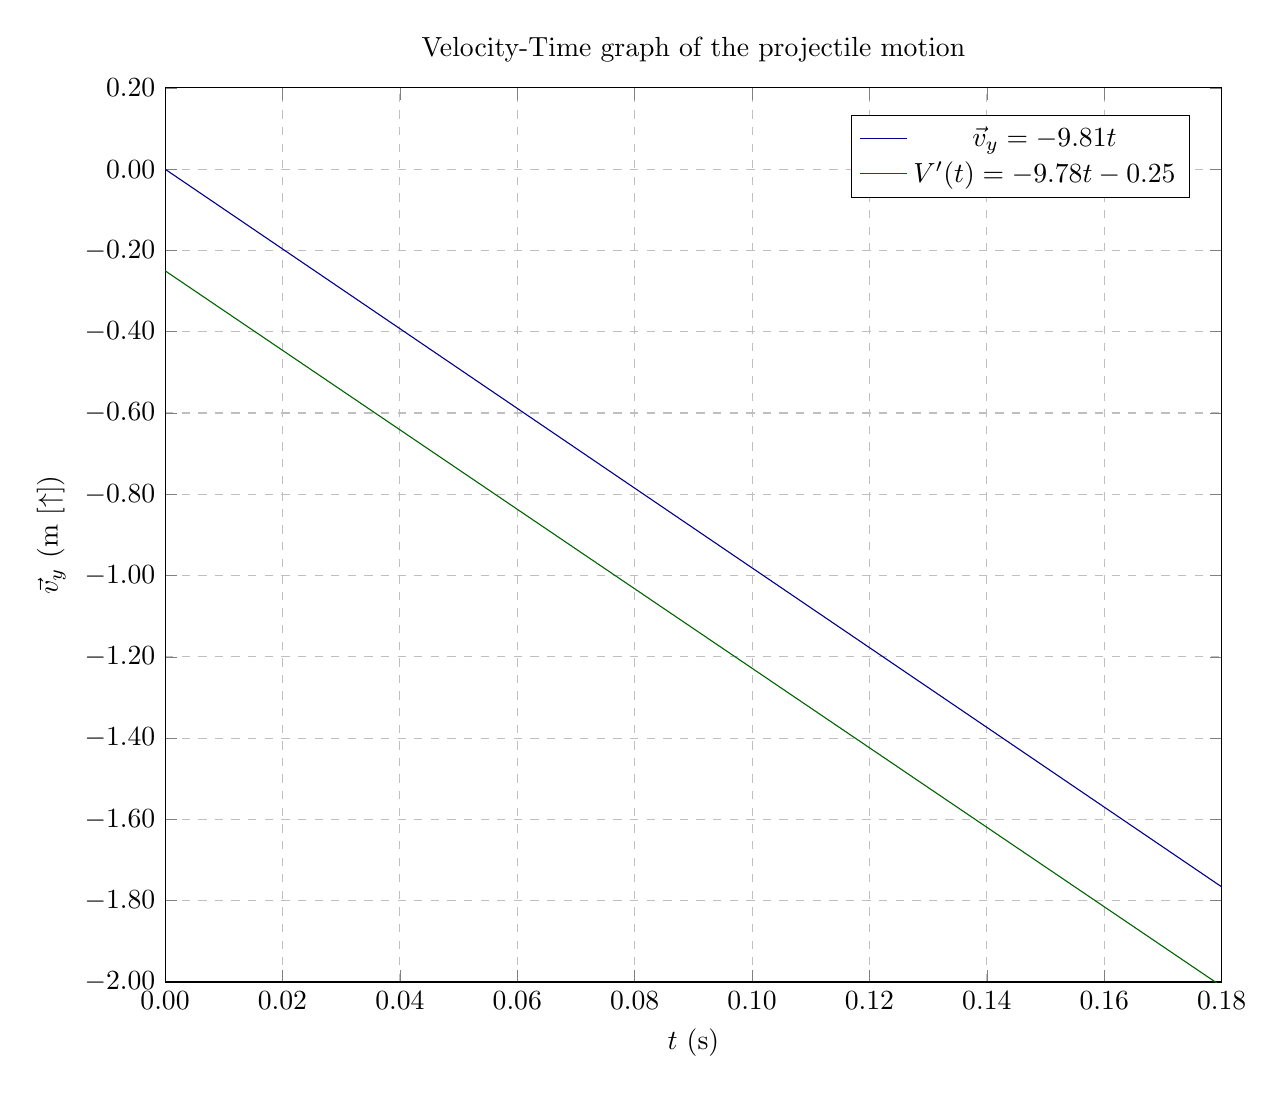
\begin{tikzpicture}
			\begin{axis} [
				title={Velocity-Time graph of the projectile motion},
				xlabel={$t$ (\text{s})},
				ylabel={$\vec{v}_y$ (\text{m} [$\uparrow$])},
				xmin=0, xmax=0.18,
				ymin=-2, ymax=0.2,
				y tick label style={/pgf/number format/fixed,
					/pgf/number format/fixed zerofill={true}},
				x tick label style={/pgf/number format/fixed,
					/pgf/number format/fixed zerofill={true}},
				xtick distance=0.02,
				ytick distance=0.2,
				ymajorgrids=true,
				xmajorgrids=true,
				grid style=dashed,
				legend pos=north east,
				]			
				\addplot[
					color=DarkBlue,
					domain=0:0.18,
				] {
					-9.81*x
				};
				\legend{$\vec{v}_y=-9.81t$, $V'(t)=-9.78t-0.25$}
				\addplot[
					color=DarkGreen,
					domain=0:0.18,
				] {
					-9.78*x-0.25
				};
			\end{axis}
		\end{tikzpicture}
	\end{center}
	
	\subsection{Error sources}
	The position-time graph has similar curves as the theoretical graph, but the values differ as the time increases.
	
	The velocity-time graph is linear like the theoretical graph, but the values differ because of errors from the position-time graph. 
	
	The small errors are created by:
	\begin{itemize}
		\item 
	\end{itemize}
	
	\subsection{Experiment optimization}
	
	\newpage
	
	\bibliographystyle{apacite}
	\bibliography{references.bib}
	
	\section{Licensing}
	\subsection{Packages}
	All \LaTeX\, packages are provided by TeX Live under the LaTeX Project Public License (LPPL).\\
	
	The \LaTeX\, typesetting system is distributed under the LaTeX Project Public License (LPPL).\\
	
	\subsection{Tools}
	The \LaTeX\, engine is provided by TeX Live under the LaTeX Project Public License (LPPL), distributed by Nixpkgs Unstable.\\
	
	The \LaTeX\, code editor is provided by TeXstudio under the GNU General Public License (GPL) version 2, distributed by Nixpkgs Unstable.\\
	
	The NixOS Linux Operating System is distributed under the GNU Lesser General Public License (LGPL) version 2.1, distributed by Nixpkgs Unstable.\\
	
	MyBib, Overleaf Learn, and Google Sheets is used for producing this document. 
	\bigskip
	\bigskip
	\begin{center}
		\textbf{Made with passion by Hadrian Lau}
	\end{center}
	
\end{document}

% Made with passion by Hadrian Lau
